% !TeX root = main.tex

\section{选题背景}

\subsection{校园绿化}

``生态环境是人类生存和发展的根基, 生态环境变化直接影响文明兴衰演替.''\cite{__2019}
中共二十大报告指出, 中国式现代化是人与自然和谐共处的现代化.
城市作为现代化的重要载体, 应该是人与人、人与自然和谐相处的美好家园.
基于人与自然和谐共生的建设理念, 习近平总书记强调, ``城市建设要以自然为美, 把好山好水好风光融入城市''.\cite{__2022}

校园是城市的重要组成部分, 其内部绿化景观自然是生态文明建设的重要组成部分.
一方面, 绿化具有一定的功能价值.
一般来说, 植被具有调节温度、增加空气湿度、隔绝噪音、防风固沙等作用.\cite{__2022-1}
清华大学校园地处中国北方, 气候干旱, 气温变化剧烈.
秋冬季节常发生风沙灾害.
同时, 校园地处繁华市区, 周边环境嘈杂.
绿化对校园生态文明建设和生活、学习环境的改善具有重要作用.
另一方面, 绿化具有一定的艺术价值.
绿色植被对人的情绪有舒缓和调节作用.
校园内丰富多样的植物与各具特色的建筑交相辉映, 极具观赏价值.

\subsection{遥感技术}

遥感是一门现代新兴技术, 可以在不与目标直接接触的情况下, 对远离目标的物体进行感测、测量和确定其物理和几何特征.
基于高空间分辨率的太空遥感平台, 对地理特征的观测数据在数量和质量以及实效性方面都能够获得远超传统观测方法的结果, 其中也包括对于地面植被情况的观测.
遥感技术的一种广泛的应用是用于衡量地表植被状况, 前人的工作中已提出许多成熟的模型或指标, 例如 NDVI 等.
借助于遥感技术, 这些指标也能够应用于衡量校园绿化状况.

\subsection{清华校园}

清华校园内的绿化广泛且植被种类丰富.
《水木湛清华 --- 清华大学校园植物》中收录的清华校园内的植物覆盖 115 科 330 属 500 种.其中按照生物学特征分类有乔木 116 种, 灌木 132 种, 草本 252 种;按照是否人工栽培分类有栽培 319 种, 野生 181 种.

不同植物的分布范围也有所不同.
例如海南常山 (Dichroa mollissima) (\cref{fig:dichroa}) 主要集中在绿园, 从南区到至善路路口可见玉簪 (Hosta plantaginea) (\cref{fig:hosta}), 雕塑园中还有人工栽培的白桦 (Betula platyphylla) (\cref{fig:betula}) 等等.

\begin{figure}
  \centering
  \subcaptionbox{海南常山\label{fig:dichroa}}{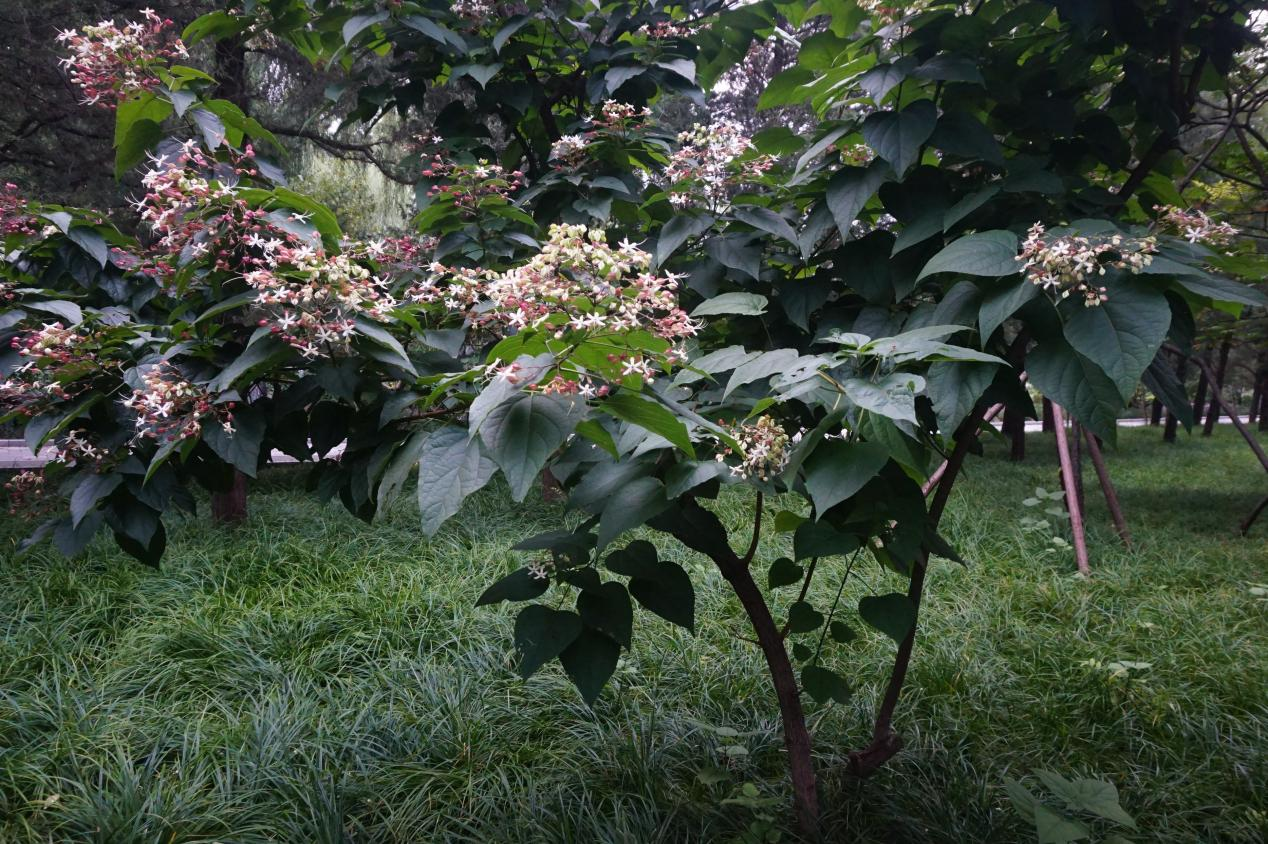
\includegraphics[height=0.3\linewidth]{assets/海南常山.png}}
  \quad
  \subcaptionbox{玉簪\label{fig:hosta}}{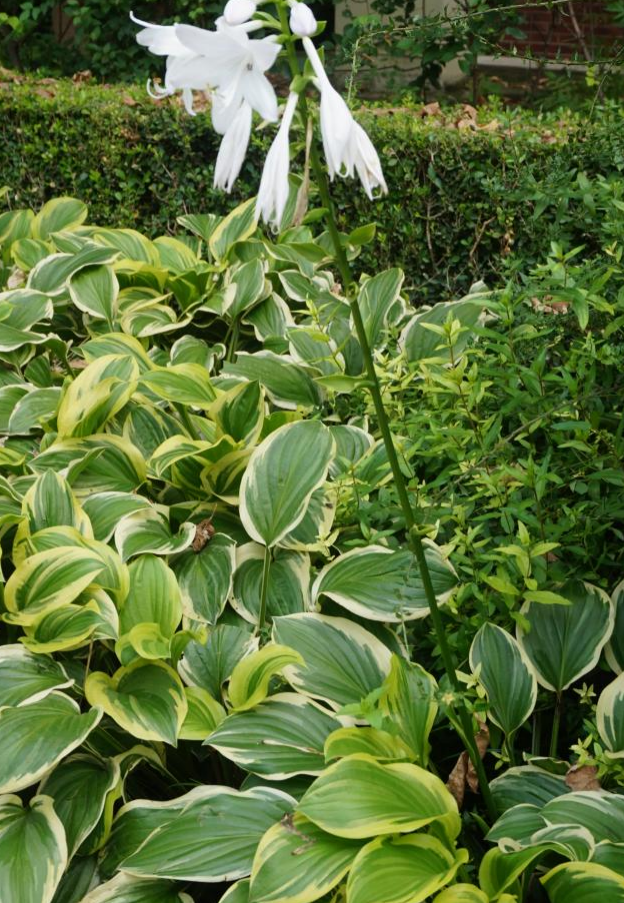
\includegraphics[height=0.3\linewidth]{assets/玉簪.png}}
  \quad
  \subcaptionbox{白桦\label{fig:betula}}{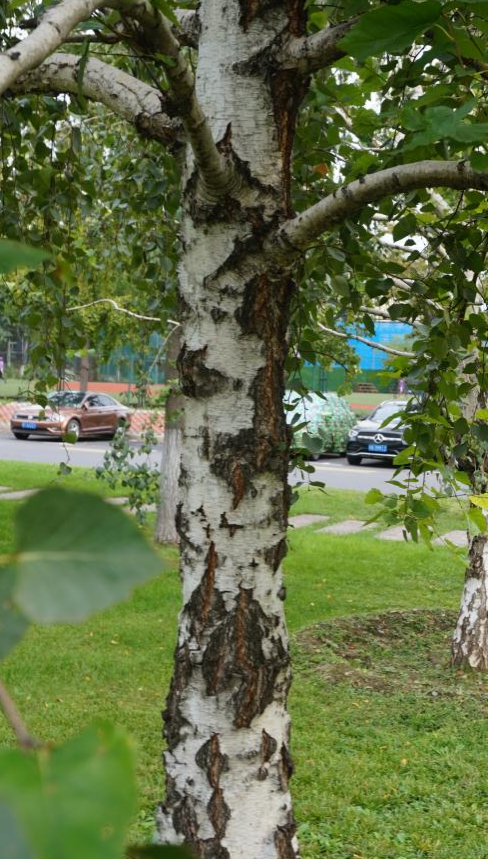
\includegraphics[height=0.3\linewidth]{assets/白桦.png}}
  \quad
  \caption{清华校园内植被}
\end{figure}

众多的植被共同丰富了清华校园的绿化环境, 对这些植被状况的监测是必不可少的.
